\chapter{玻色弦及其量子化}
\label{chap:2}
本章简要回顾玻色弦的量子化,虽然玻色弦有诸如真空不稳定以及没有费米子激发等问题,但对玻色弦的研究有助于理解超弦的相关问题。这里只做简要的回顾,更多相关细节读者可以参考\cite{Polchinski:1998rq,Blumenhagen:2013fgp,Becker:2006dvp},另外我们将使用更现代的共形场论的语言,相关细节可以在\cite{DiFrancesco:1997nk,Blumenhagen:2009zz}中找到。

\section{正则量子化}
弦论量子化其实是约束体系量子化问题,利用正则量子化并不能很好地解决,但是正则量子化的好处是能看出弦论的粒子谱。
\subsection{Nambu-Goto 作用量}
自由点粒子的作用量正比于其世界线场,受此启发可以立刻写下弦的作用量:
\begin{equation}
	S_{\text{NG}}=-\frac{1}{2\pi\alpha^\prime}\int_M d\tau d\sigma \left(\det h_{ab}\right)^{1/2},\quad h_{ab}:=\partial_a X^\mu \partial_b X_\mu
\end{equation}
由于作用量中包含根号,更利于量子化的方式是引入辅助场$\gamma_{ab}$
\begin{equation}
	\label{eq:2.2}
	S_\mathrm{P}[X,\gamma]=-\frac{1}{4\pi\alpha^{\prime}}\int_Md\tau d\sigma\left(-\gamma\right)^{1/2}\gamma^{ab}\partial_aX^\mu\partial_bX_\mu
\end{equation}
上述作用量有全局庞加莱对称性:
\begin{equation}
	\begin{aligned}&X^{\prime\mu}(\tau,\sigma)=\Lambda_{\nu}^{\mu}X^{\nu}(\tau,\sigma)+a^{\mu},\\&\gamma_{ab}^{\prime}(\tau,\sigma)=\gamma_{ab}(\tau,\sigma).\end{aligned}
\end{equation}
以及局域规范对称性$\mathrm{diff}\times\mathrm{Weyl}$:
\begin{equation}
	\begin{aligned}
		X^{\prime}{}^{\mu}(\tau^{\prime},\sigma^{\prime})&=X^{\mu}(\tau,\sigma),\\ \frac{\partial\sigma^{\prime c}}{\partial\sigma^a}\frac{\partial\sigma^{\prime a}}{\partial\sigma^b}\gamma_{cd}^{\prime}(\tau^{\prime},\sigma^{\prime})&=\gamma_{ab}(\tau,\sigma),
	\end{aligned}
\end{equation}
	
\begin{equation}
	\begin{aligned}
		X^{\prime\mu}(\tau,\sigma)&=X^\mu(\tau,\sigma),\\\gamma_{ab}^{\prime}(\tau,\sigma)&=\exp(2\omega(\tau,\sigma))\gamma_{ab}(\tau,\sigma),
	\end{aligned}
\end{equation}
由于$\gamma_{ab}$没有动力学,其运动方程将在量子化时作为约束引入:
\begin{equation}
	\label{eq:2.6}
	\frac{\delta S_\mathrm{P}}{\delta \gamma_{ab}}\sim T^{ab}=0
\end{equation}
同时不难验证弦经典运动方程为一维波动方程:
\begin{equation}
		\frac{\delta S_\mathrm{P}}{\delta X^\mu}\sim\left(\frac{\partial^2}{\partial\sigma^2}-\frac{\partial^2}{\partial\tau^2}\right)X^\mu=0
\end{equation}
由于一维弦的非平凡拓扑,若加入周期性边界条件则为闭弦:
\begin{equation}
	\label{eq:2.8}
	X^\mu(\tau,\sigma+\ell) = X^\mu(\tau,\sigma)
\end{equation}
而开弦端点上可以引入两种不同的边界条件:
\begin{equation}
	\label{eq:2.9}
	\begin{aligned}
	&	\left.n^a\partial_aX_\mu\right|_{\partial M}=0\quad \text{(Neumann)}\\
	&	X^\mu(\tau,0)=X^\mu(\tau,\ell)=x_0\quad \text{(Dirichlet)}
	\end{aligned}
\end{equation}
表面上看似乎只有第一种边界条件才不会破坏庞加莱对称性,Dirichlet边界条件其实相当于要求开弦端点依附于D膜上。而超弦中D膜其实可以作为BPS态稳定存在,所以D膜作为靶空间的非平凡缺陷也应当看作弦论自由度的一部分,这意味着Dirichlet边界条件也是可行的。

弦论中可以通过Chan-Paton因子引入$U(N)$规范对称性\footnote{非定向弦对应$SO(N)$和$Sp(N)$对称性},具体体现在开弦端点带上$U(1)\times \bar U(1)$荷,其可以解释为开弦端点依附的D膜指标:
\begin{equation}
	|N;k;a\rangle=\sum_{i,j=1}^n|N;k;ij\rangle\lambda_{ij}^a,\quad \lambda\in \mathfrak{u}(N)
\end{equation}
\subsection{光锥量子化}
正则量子化的核心是将力学量量子化为算符,泊松括号替换为狄拉克括号。但是量子化还要满足约束\ref{eq:2.6}。光锥量子化思路是取光锥规范定下$\mathrm{diff}\times\mathrm{Weyl}$规范对称性,类似在库伦规范下量子化$U(1)$Yang-Mills理论得到量子电动力学:
\begin{equation}
	\begin{gathered}
		X^\pm=2^{-1/2}(X^0\pm X^1),\quad X^i,i=2,\ldots,D-1\\
		X^+=\tau,\quad\partial_\sigma\gamma_{\sigma\sigma}=0,\quad\det\gamma_{ab}=-1
	\end{gathered}
\end{equation}
在这一规范选取下,$X^{+}$不再拥有动力学演化,而$X^{-}$可以完全由横向$\alpha^i$模展开,所以$\alpha^-$也不用考虑。以Neumann边界条件开弦为例,仅剩下非平凡的$X^i$模展开:
\begin{equation}
	\label{eq:2.12}
	X^i(\tau,\sigma)=x^i+\frac{p^i}{p^+}\tau+i(2\alpha^{\prime})^{1/2}\sum_{n=-\infty}^\infty\frac{1}{n}\alpha_n^i\exp\left(-\frac{\pi in\tau}{\ell}\right)\cos\frac{\pi n\sigma}{\ell}
\end{equation}
这里$x$可以理解为弦的质心动量,$p,\Pi$是相应的共轭动量:
\begin{equation}
	\begin{gathered}
		x^-(\tau)=\frac{1}{\ell}\int_0^\ell d\sigma X^-(\tau,\sigma)\\
		p_-=-p^+=\frac{\partial L}{\partial(\partial_\tau x^-)}=-\frac{\ell}{2\pi\alpha^{\prime}}\gamma_{\sigma\sigma}\\
		\Pi^i=\frac{\partial L}{\partial(\partial_\tau X^i)}=\frac{1}{2\pi\alpha^{\prime}}\gamma_{\sigma\sigma}\partial_\tau X^i=\frac{p^+}{\ell}\partial_\tau X^i
		x^i(\tau)=\frac{1}{\ell}\int_0^\ell d\sigma X^i(\tau,\sigma),\\p^i(\tau)=\int_0^\ell d\sigma\Pi^i(\tau,\sigma)=\frac{p^+}{\ell}\int_0^\ell d\sigma\partial_\tau X^i(\tau,\sigma)
	\end{gathered}
\end{equation}
然后取等时对易子进行标准正则量子化操作:
\begin{equation}
	\begin{aligned}
		[x^-,p^+]&=i\eta^{-+}=-i ,\\
		[X^i(\sigma),\Pi^j(\sigma^{\prime})]&=i\delta^{ij}\delta(\sigma-\sigma^{\prime}) 
	\end{aligned}
	\quad\Rightarrow\quad
	\begin{aligned}
		[x^i,p^j]&=i\delta^{ij} ,\\
		[\alpha_m^i,\alpha_n^j]&=m\delta^{ij}\delta_{m,-n}
	\end{aligned}
\end{equation}
不难看出上面模展开具有谐振子代数,所以弦的粒子谱可以看作不同振动模式激发:
\begin{equation}
	|N;k\rangle=\left[\prod_{i=2}^{D-1}\prod_{n=1}^\infty\frac{(\alpha_{-n}^i)^{N_{in}}}{(n^{N_{in}}N_{in}!)^{1/2}}\right]|0;k\rangle
\end{equation}
其中$\ket{0,k}$是真空态,且由于$p^i$为好量子数而带有背景动量。利用黎曼Zeta正规化$\zeta(-1)=-\frac{1}{12}$可以推出点粒子激发质量谱为:
\begin{equation}
	\label{eq:2.16}
	m^2_\mathrm{op}=\frac{1}{\alpha^{\prime}}\left(N+\frac{2-D}{24}\right),\quad N:=\sum_{i=2}^{D-1}\sum_{n=1}^{\infty}nN_{in}
\end{equation}
但是光锥量子化方法明显地破坏了庞加莱对称性,为了理论自洽,必须要求玻色弦定义在$26$维靶空间:
\begin{equation}
	\boxed{
		D_{\text{boson}}=26
	}
\end{equation}
这其实是第一激发态处于$SO(D-2)$小群表示的必然结果。注意到弦真空是质量平方负定的快子态:
\begin{equation}
	|0;k\rangle\Leftrightarrow m^2=-\frac{1}{\alpha^\prime}
\end{equation}
闭弦也可以同样处理,只是分为左右模,而开弦左右模叠加成为驻波\ref{eq:2.12},闭弦有如下模展开:
\begin{equation}
	\label{eq:2.19}
	\begin{aligned}X^i(\tau,\sigma)&=x^i+\frac{p^i}{p^+}\tau+i\left(\frac{\alpha^{\prime}}{2}\right)^{1/2}\\&\times\sum_{n=-\infty}^\infty\left\{\frac{\alpha_n^i}{n}\exp\left[-\frac{2\pi in(\sigma+\tau)}{\ell}\right]+\frac{\tilde{\alpha}_n^i}{n}\exp\left[\frac{2\pi in(\sigma-\tau)}{\ell}\right]\right\}\end{aligned}
\end{equation}
可以看到相当于两个开弦谱的叠合。同样正则量子化得到弦激发粒子谱:
\begin{equation}
	|N,\tilde{N};k\rangle=\left[\prod_{i=2}^{D-1}\prod_{n=1}^\infty\frac{(\alpha_{-n}^i)^{N_{in}}(\tilde{\alpha}_{-n}^i)^{\tilde{N}_{in}}}{(n^{N_{in}}N_{in}!n^{\tilde{N}_{in}}\tilde{N}_{in}!)^{1/2}}\right]|0,0;k\rangle
\end{equation}
闭弦周期性边界条件要求左右模满足$N=\tilde{N}$\footnote{注意这一条件并非总是满足,对于T紧致化后的靶空间,左右模间可以相差缠绕数。}。同样可以得到闭弦质量谱:
\begin{equation}
	m^2_{\mathrm{cl}}=\frac{2}{\alpha^\prime}(N+\tilde{N}-2)=\frac{4}{\alpha^\prime}(N-1)
\end{equation}
本论文主要考察无质量激发态,也就是开弦闭弦第一激发态,事实上更高激发态在$\alpha^\prime\to0$的场论极限下会被压低。从上面的弦粒子谱不难看出开弦第一激发态对应无质量规范玻色子,而闭弦第一激发态对应引力子,伸缩子以及$B$-场。
\subsection{协变量子化}
光锥量子化相当于先取规范使用约束条件后量子化,协变量子化相当于先量子化后使用约束条件,好处是明显地保留了庞加莱对称性。下面仍以开弦为例,好处是左右模重合。

要求$T_{ab}=0$从物理上看应当是要求其作用于量子化后的希尔伯特空间上是零算子:
\begin{equation}
	\label{eq:2.22}
	T_{ab}=0\xrightarrow{\text{量子化}} T_{ab}\ket{\psi}=0\Rightarrow L_n^m\ket{\psi}\sim0
\end{equation}
其中$L_n$是能动张量模展开后的Virasoro代数生成元:
\begin{equation}
	L_m=\frac{1}{2}\sum_{n=-\infty}^{+\infty}\alpha_{m-n}\cdot\alpha_n
\end{equation}
上述条件相当于要求物理态为Virasoro最高权态\footnote{$A$是待定常数,不少文献称为正规排序常数,计算上来源于NOP序和产生湮灭算符排序之间相差的常数。本质上来源于真空能贡献。}:
\begin{equation}
	\label{eq:2.23}
	(L_n^\mathrm{~m}+A\delta_{n,0})|\psi\rangle=0\quad\mathrm{for~}n\geq0
\end{equation}
由于不用选取光锥规范,\ref{eq:2.12}\ref{eq:2.19}中模展开应当将指标$i$替换为一般的$\mu$,现在态空间由$\alpha^\mu$生成。\ref{eq:2.23}的限制并不够,因为$\mathscr{H}_{\mathrm{phys}}$中还包含一些零模态,与物理态均正交,张成的希尔伯特空间记为$\mathscr{H}_{\mathrm{null}}$,所以和物理过程是解耦的,应当看作是规范变换的生成元,所以应当有下面的等价关系:
\begin{equation}
	\ket\psi \sim \ket\psi +\ket\chi,\quad \forall\psi\in\mathscr{H}_{\mathrm{phys}},\chi\in\mathscr{H}_{\mathrm{null}}
\end{equation}
最终我们得到协变微扰论的态空间:\footnote{这里似乎很像BRST量子化\ref{eq:2.48},但是由于我们并没有直接考虑鬼场,所以无法写下一个分次链复形}
\begin{equation}
	\label{eq:2.26}
	\mathscr{H}_{\mathrm{CQ}}\simeq\frac{\mathscr{H}_{\mathrm{phys}}}{\mathscr{H}_{\mathrm{null}}}
\end{equation}
计算此商空间便得到弦的激发态,而且自洽性自然要求$A=-1,D=26$,开弦快子态和无质量激发态构造如下:
\begin{equation}
	\begin{gathered}
		|0;k\rangle,\quad m^2=-\frac{1}{\alpha^{\prime}};\\e_{\mu}\alpha_{-1}^\mu|0;k\rangle,\quad m^2=0,k^\mu e_{\mu}=0,\\e_{\mu}\cong e_{\mu}+c k_\mu.
	\end{gathered}
\end{equation}
同时叠合关系给出闭弦激发态为:
\begin{equation}
	\begin{gathered}
		|0;k\rangle,\quad m^2=-\frac{4}{\alpha^{\prime}};\\e_{\mu\nu}\alpha_{-1}^\mu\tilde{\alpha}_{-1}^\nu|0;k\rangle,\quad m^2=0,k^\mu e_{\mu\nu}=k^\nu e_{\mu\nu}=0,\\e_{\mu\nu}\cong e_{\mu\nu}+a_\mu k_\nu+k_\mu b_\nu,a\cdot k=b\cdot k=0.
	\end{gathered}
\end{equation}
好处是态的构造明显保留庞加莱对称性,从而为计算Lorentz不变的弦振幅带来了方便。
\section{路径积分量子化}
不同于量子场论,弦论的相互作用并不需要在作用量中引入新的项来实现,而是直接由不同的世界面拓扑来实现。
\subsection{Polyakov路径积分}
为了使路径积分良定,先利用Wick转动将世界面度规从$(-,+)$的二维闵氏度规$\gamma_{ab}$转为$(+,+)$的二维欧式度规$g_{ab}$。单纯从$\mathrm{diff}\times\mathrm{Weyl}$不变性出发可以在\ref{eq:2.2}基础上额外引入一项正比于:
\begin{equation}
	\chi=\frac{1}{4\pi}\int_Md^2\sigma\mathrm{~g}^{1/2}R+\frac{1}{2\pi}\int_{\partial M}dsk
\end{equation}
其中$k$是测地曲率,利用Gauss-Bonnet定理不难看出这一项正是欧拉示性数。由于二维几何均共形平坦,所以可以选取等温坐标使得:
\begin{equation}
	\label{eq:2.30}
	g = \mathrm{e}^{2\omega} dz d\bar z
\end{equation}
再利用Weyl不变性可以将其变为平坦欧氏度规,也即选取共形规范。在这一规范下\footnote{用$\hat g$表示对应的规范固定选取。},利用Faddeev–Popov方法引入费米统计的$b,c$鬼场消去$\mathrm{diff}\times\mathrm{Weyl}$规范冗余,弦论配分函数可以写作:
\begin{equation}
	\label{eq:2.31}
	Z\left[\hat{g}\right]=\sum_{\substack{\text{worldsheet}\\\text{topologies}}}\frac{1}{V_{\mathrm{CKG}}}\int\mathcal{D}X\mathcal{D}[b\tilde{b}]\mathcal{D}[c\tilde{c}]\exp(-S_m-S_\mathrm{g})
\end{equation}
这里物质场和鬼场作用量分别为:
\begin{equation}
	\label{eq:2.32}
	\begin{aligned}
		S_m&=\frac{1}{2\pi\alpha^{\prime}}\int d^2z\mathrm{~}\partial X^\mu\bar{\partial}X_\mu,\quad
		S_g&=\frac{1}{2\pi}\int d^2z\left(b\bar\partial c+\tilde b\partial \tilde c\right)
	\end{aligned}
\end{equation}
注意$\mathrm{diff}\times\mathrm{Weyl}$规范固定后其实还剩下共形规范自由度没有消去\footnote{对高亏格曲面其实还会有额外的零模鬼场插入,这里留待第\ref{chap:4}章讨论},所以这时$S_m$和$S_g$都对应二维共形场论。所以弦论问题就被转化为了二维共形场论问题。而且可以看到弦论中的展开不同于量子场论中按照顶点数目展开,弦论是按照拓扑展开,相互作用系数有如下关系:
\begin{equation}
	g_0^2\thicksim g_c\thicksim e^\lambda
\end{equation}

注意,对于开弦,由于端点的世界线会构成世界面的边界,所以开弦实际上需要使用边界共形场论进行研究。此时左右模均定义在上半复平面上,而且Neumann边界条件\footnote{鬼场也会有类似的限定}体现在实轴上左右模的对应:
\begin{equation}
	T(z)=\tilde{T}(\bar{z}),\quad c(z)=\tilde{c}(\bar{z}),\quad b(z)=\tilde{b}(\bar{z}),\quad\operatorname{Im}z=0
\end{equation}
这时只能在上复平面讨论共形场论,不过可以用加倍技巧将上复平面右模的信息转移到下复平面左模场的定义:
\begin{equation}
	\label{eq:2.35}
	T(z):= \tilde T(\bar{z}^{\prime}),b(z):= \tilde b(\bar{z}^{\prime}),c(z):= \tilde c(\bar{z}^{\prime})\quad z^\prime = \bar z,\mathrm{Im}z<0
\end{equation}
对左模场延拓\footnote{这种延拓技巧在数学上依赖于Schwarz反射原理}之后左模场已然包含右模场的所有信息,所以可以转换为在整个复平面上仅仅讨论左模场的共形场论。下面的简单例子便能说明加倍技巧:
\begin{equation}
	\begin{aligned}
		L_m&=\frac{1}{2\pi i}\int_C\left(dzz^{m+1}T(z)-d\bar{z}\bar{z}^{m+1}\tilde{T}(\bar z)\right)
		\\&=\frac{1}{2\pi i}\oint dzz^{m+1}T(z)
	\end{aligned}
\end{equation}
开弦左右模重叠,围道积分由于边界的限制只能在上复平面进行。利用加倍技巧将右模的信息转换为左模在下复平面上的信息,从而将边界共形场论转换为一般的共形场论,而且只剩下左模场参与计算。所以闭弦和开弦的计算是一样的,只需要注意开弦只保留左模,或者简单认为左右模场此时相等\footnote{但是注意严谨来讲边界条件只给出实轴上相等,是利用加倍技巧之后才在复平面上等同,而且这种分析技巧只适用于复平面,对于本文主要讨论的树级振幅已足够。}。

另外,根据二维闭曲面分类定理,对世界面拓扑求和也可以是不可定向曲面,对不可定向曲面求和意味着我们将世界面宇称$\sigma^{\prime}=\ell-\sigma^2$作为规范对称性引入。这时的弦论成为不可定向弦。考虑世界面宇称变换由$\Omega$算符生成,对于开弦有:
\begin{equation}
	\Omega\alpha_n^\mu\Omega^{-1}=(-1)^n\alpha_n^\mu
\end{equation}
而对于闭弦则会左右模互换:
\begin{equation}
	\Omega\alpha_n^\mu\Omega^{-1}=\tilde\alpha_n^\mu,\quad \Omega\tilde\alpha_n^\mu\Omega^{-1}=\alpha_n^\mu
\end{equation}
且假设真空态$\Omega=+1$,在这一约定下,自洽的弦相互作用要求不可定向弦只剩下$\Omega=+1$的激发态。本论文主要考虑可定向弦的树级振幅计算。
\subsection{弦振幅}
类似量子场论中振幅依赖于渐进态的定义,弦论中我们提到振幅都是指无穷远处的弦激发态演化后的相互作用关联函数。取等温坐标后,利用共形场论的态算符对应,无穷远处的激发态相当于世界面某个点上插入对应的顶角算符$\mathscr{V}$,用图示来看这个过程相当于图\ref{fig:1}。
\begin{figure}[htbp]
	\centering
	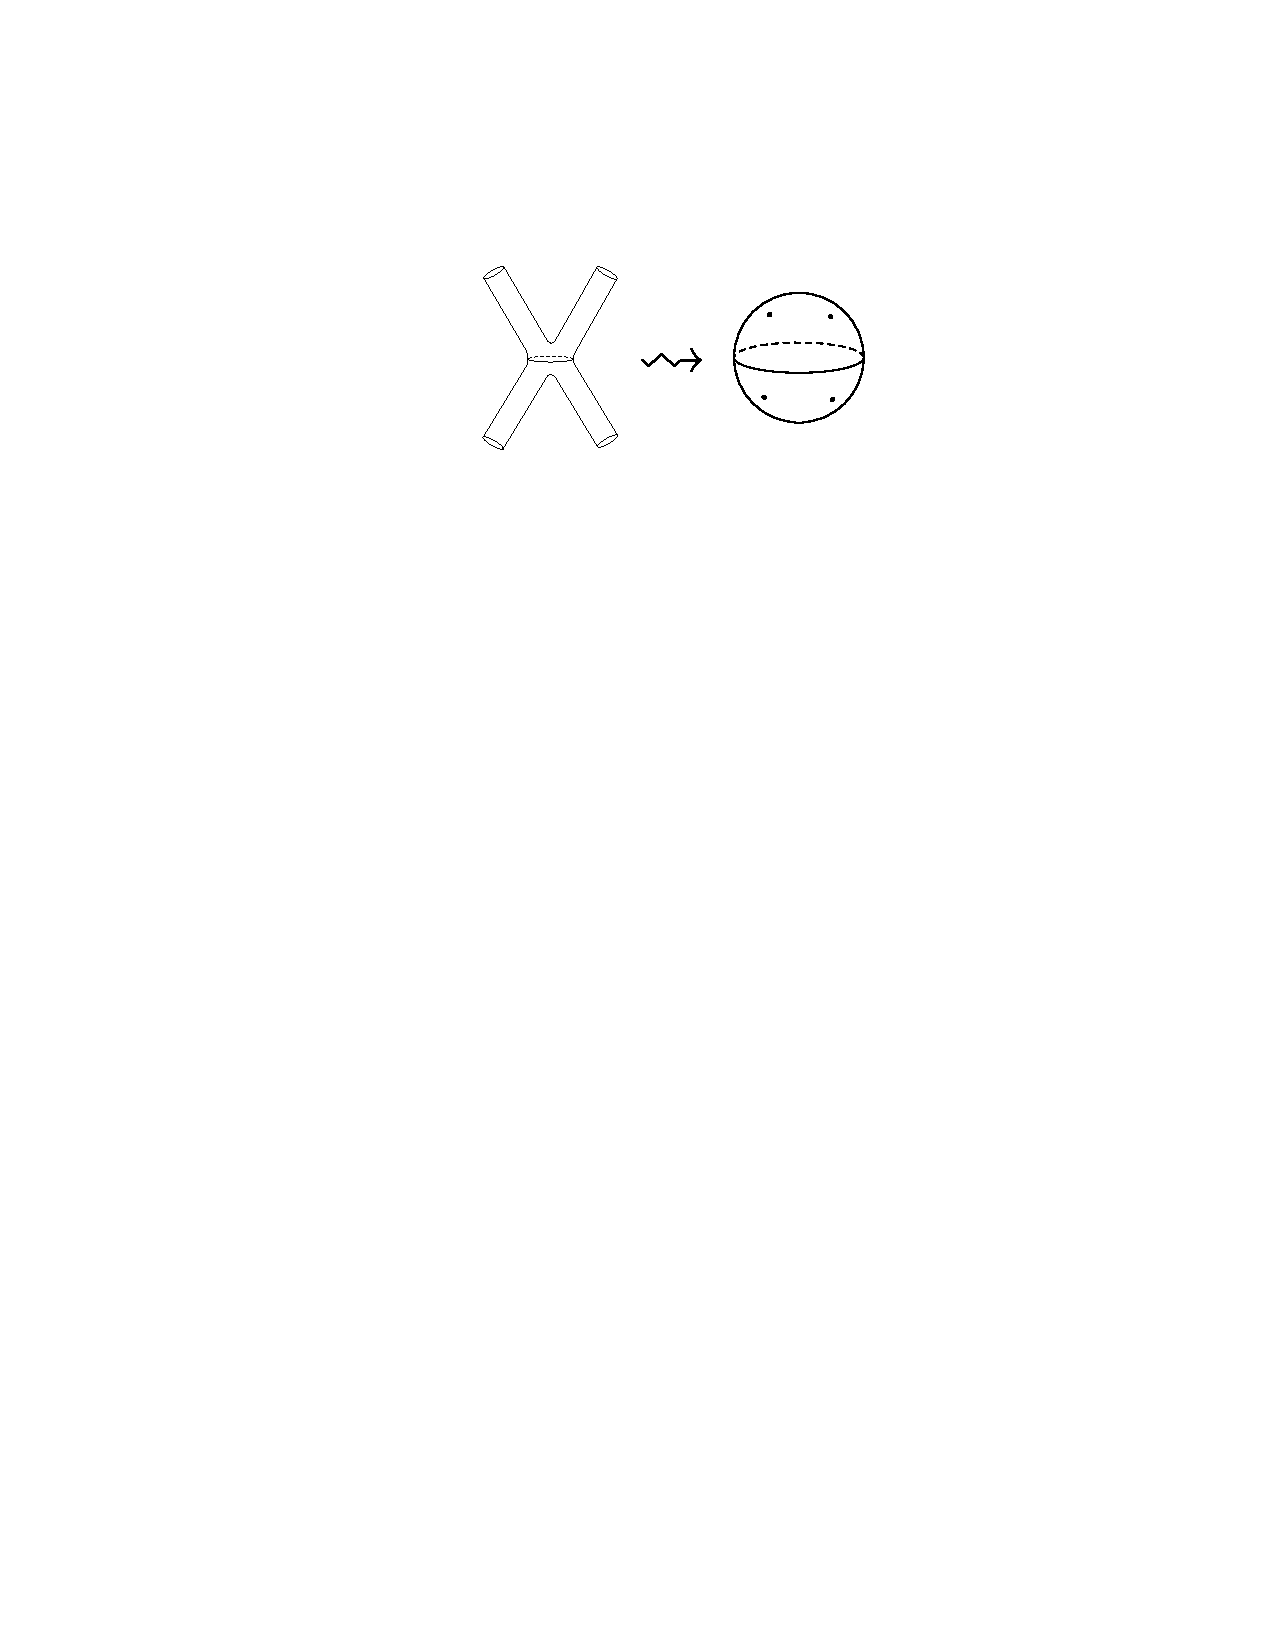
\includegraphics{figs/fig1.pdf}
	\caption{态算符对应与弦振幅}
	\label{fig:1}
\end{figure}
受前面配分函数的启发,由此可以写下弦振幅\footnote{也称作弦的S矩阵。}:
\begin{equation}
	\label{eq:2.39}
	\begin{aligned}
		S_{j_1...j_n}(k_1,\ldots,k_n)&=\llangle[\Big]\prod_{i=1}^n\int d^2\sigma_ig(\sigma_i)^{1/2}\mathscr{V}_{j_i}(k_i,\sigma_i)\rrangle[\Big]
		\\&=\sum_{\substack{\text{worldsheet}\\\text{topologies}}}\mathrm{e}^{-\lambda \chi}\int\frac{\mathcal{D}X\mathcal{D}g}{V_{\mathrm{diff}\times\mathrm{Weyl}}}\mathrm{e}^{-S_m}\prod_{i=1}^n\int d^2\sigma_ig(\sigma_i)^{1/2}\mathscr{V}_{j_i}(k_i,\sigma_i)
	\end{aligned}
\end{equation}
上式中我们使用$\llangle\bullet\rrangle$是为了提醒读者规范固定时可能的零模鬼场插入。而且上式我们并没有利用鬼场进行规范固定,这个问题我们留待到第\ref{chap:4}章解决。
\subsection{顶角算符}
利用前面正则量子化得到的激发态,只需要做如下替换便可以得到对应的顶角算符:
\begin{equation}
	\alpha_{-m}^\mu\to i\left(\frac{2}{\alpha^{\prime}}\right)^{1/2}\frac{1}{(m-1)!}\partial^mX^\mu(0),\quad
	|0;k\rangle\rightarrow e^{ik\cdot X(0,0)}
\end{equation}
由于算符乘积展开(OPE)在插入点相同时奇异,所以替换完成后还需要对算符取正规排序乘积(NOP)保证非奇异。这其实相当于一种重整化的选取,本论文均采用共形场论的NOP技术来重整化。

一般我们把上述构造的算符与世界面上积分$\int d\sigma^2$\footnote{注意开弦由于插入点在边界上,所以积分在边界上进行。}共同称作积分顶角算符,记作$U$,积分的存在使得顶角算符整体共形权为$0$,从而最终的振幅具有共形不变性。
\section{BRST量子化}
本节的核心目标是使用BRST量子化方法给出后续振幅计算中规范固定需要引入的无积分顶角算符。

考虑关于物质场$\phi_i$的某个一般性量子理论,$i$以及后续讨论涉及到的指标可以连续或离散,连续部分标记场的坐标依赖,离散部分则标记场的种类。假设所考虑体系的规范对称性生成元$\delta_\alpha$具有类似李代数的结构:
\begin{equation}
	\label{eq:2.41}
	[\delta_\alpha,\delta_\beta]=f_{\alpha\beta}^\gamma\delta_\gamma
\end{equation}
利用FP方法引入鬼场进行规范固定,规范选取为:
\begin{equation}
	F^A(\phi)=0
\end{equation}
则配分函数计算为:
\begin{equation}
	\int\frac{[d\phi_i]}{V_{\mathrm{gauge}}}\exp(-S_1)\to\int[d\phi_idB_Adb_Adc^\alpha]\exp(-S_m-S_g-S_f)
\end{equation}
这里新引入了鬼场$S_g$和规范固定项$S_f$:\footnote{前面\ref{eq:2.31}没有$S_f$是因为规范选取完全消除了$g$的规范冗余,不难看到$B_A$积分后的效果是引入$\delta(F^A(\phi))$,所以对$g$再次进行路径积分便完全移除了这一项。}
\begin{equation}
	S_g=b_Ac^\alpha\delta_\alpha F^A(\phi),\quad S_f=-iB_AF^A(\phi)
\end{equation}
以上无非是FP鬼场的一般做法,重点在于上述体系存在一个全局对称性:
\begin{equation}
	\begin{aligned}
		\delta_{\mathbf{B}}\phi_i 
		&= -i\epsilon c^\alpha\delta_\alpha\phi_i,  
		& \quad \delta_{\mathbf{B}}B_A 
		&= 0, \\
		\delta_{\mathbf{B}}b_{A} 
		&= \epsilon B_A,  
		& \quad \delta_{\mathbf{B}}c^{\alpha} 
		&= \frac{i}{2}\epsilon f^\alpha{}_{\beta\gamma} c^\beta c^\gamma.
	\end{aligned}
\end{equation}
对应的Noether荷记作$Q_B$,其中$\epsilon$是格拉斯曼变量。$c$的鬼数为$+1$,$b$和$\epsilon$鬼数为$-1$。所以$Q_B$具有$+1$的鬼数,而且具有幂零性:
\begin{equation}
	Q_{\mathrm{B}}^2=0
\end{equation}
考虑物质场和鬼场共同生成的希尔伯特空间,以鬼数为分次可以立即写下BRST上链复形$C^{\bullet}_{\mathrm{BRST}}$:
\begin{equation}
	\cdots\longrightarrow\mathscr{H}_{g-1}\xrightarrow{Q_{g-1}}\mathscr{H}_g\xrightarrow{Q_g}\mathscr{H}_{g+1}\longrightarrow\cdots
\end{equation}
BRST量子化则是要求物理态处于鬼数为0的上同调群中\footnote{对于无积分顶角算符则是要求在鬼数为1的上同调群中,而且额外要求是共形不变的,也就是限制在共形权为0的子复形中讨论上同调。},这其实是要求可观测量具有BRST不变性:\footnote{准确来说$\ket{\text{phys}}\in Z$,闭链要求给出BRST不变性,而模掉边缘链$B$(物理上也称$B$中的态为BRST恰当)意味着$B$中的态都是和物理态脱耦的,类似\ref{eq:2.26}}
\begin{equation}
	\label{eq:2.48}
	\mathscr{H}_{\mathrm{BRST}}\cong H^0(C^\bullet_{\mathrm{BRST}}):=Z(C^\bullet_{\mathrm{BRST}})/B(C^\bullet_{\mathrm{BRST}})
\end{equation}

接下来我们将上面一般性的方法应用到弦论中,BRST荷有如下形式:
\begin{equation}
	\label{eq:2.49}
	Q_B=\frac{1}{2\pi i}\oint(\operatorname{d}zj_B-\operatorname{d}\overline{z}\tilde{j}_B),\quad
	j_{\mathrm{B}}:=cT^m+:bc\partial c:+\frac{3}{2}\partial^2c
\end{equation}
$Q_B^2=0$要求$\{Q_B,Q_B\}=0$,这对应$j_B$OPE的一阶奇点:\footnote{这些复杂的OPE计算可以使用笔者编写的程序完成:\url{https://github.com/WHUZBF/MMA/tree/main/OPE}}
\begin{equation}
	j_B(z)j_B(w)\sim-\frac{c^m-18}{2(z-w)^3}c\partial c(w)-\frac{c^m-18}{4(z-w)^2}c\partial^2c(w)-\frac{c^m-26}{12(z-w)}c\partial^3c(w)
\end{equation}
由此可以看出自洽量子化要求$c^m=26$,也即靶空间维数为$26$。另外,物理态在壳要求:
\begin{equation}
	\label{eq:2.51}
	L_0|\psi\rangle=\{Q_B,b_0\}|\psi\rangle=0\Rightarrow b_0\ket{\psi}=0
\end{equation}
为了构造无质量态无积分顶角算符,首先使用$bc$鬼场物质场$\partial^n X$以及平面波$\mathrm{e}^{ip\cdot X}$构造出最一般的共形权为$0$的顶角算符:\footnote{注意我们这里忽视了鬼数为1这个条件,后面会在求BRST恰当项中引入。也可以先引入这个条件使得计算更加简便,但我们这里考虑最一般的构造帮助读者熟悉OPE计算。}
\begin{equation}
	V_{\text{general}}=:\left(\alpha\partial c+\beta c\partial^2c+\gamma c\partial c\partial^2c+\epsilon_\mu c\partial X^\mu+\zeta_\mu c\partial c\partial X^\mu+\lambda\right)e^{ip\cdot X}:
\end{equation}
上述对态的要求可以转化为对算符的要求:\footnote{这里我们利用了$Q$的定义含围道积分,对易子的计算可以转换为被积算符OPE的计算}
\begin{equation}
	Q_B\ket{\psi}=0\Leftrightarrow [Q_B,V] = 0 \Leftrightarrow Q_B V\sim 0
\end{equation}
首先作用在壳条件得到:
\begin{equation}
	\begin{aligned}
		&\begin{aligned}
		b_0V_{\text{general}}&=\oint\frac{\mathrm{d}z}{2\pi i}zb:\left(\alpha\partial c+\beta c\partial^2c+\gamma c\partial c\partial^2c+\epsilon_\mu c\partial X^\mu+\zeta_\mu c\partial c\partial X^\mu+\lambda\right)e^{ip\cdot X}:\\
		&=\oint\frac{\mathrm{d}z}{2\pi i}:\left(\frac{\alpha}{z}-\frac{\gamma c\partial^2c}{z}-\frac{\zeta_\mu(c\partial X^\mu)}{z}\right)e^{ip\cdot X}:=0\\
	\end{aligned}\\
	&\Rightarrow\alpha,\gamma,\zeta^\mu = 0
	\end{aligned}
\end{equation}
剩下的可能的顶角算符形式为:
\begin{equation}
	V_{\text{general}}\to V_1=:\left(\beta c\partial^2c+\epsilon_\mu c\partial X^\mu+\lambda\right)e^{ip\cdot X}:
\end{equation}
继续作用式\ref{eq:2.49},注意这里考虑开弦,只有左模:
\begin{equation}
	\begin{aligned}
		&Q_BV_1=\oint\frac{\mathrm{d}z}{2\pi i}\left[-\frac{i\alpha^{\prime}}{4z}\epsilon\cdotp:\partial^2ce^{ip\cdot X}c:+\frac{\lambda}{z}c\partial e^{ip\cdot X}\right]=0\\
	&\Rightarrow\lambda=0,\quad\epsilon\cdot p=0
	\end{aligned}
\end{equation}
注意到BRST算符并不改变共形权,所以BRST恰当部分应当也由$V_{\text{general}}$中的项生成,另外注意到鬼数为1的恰当项应当由鬼数为0的部分生成,而鬼数为零的算符只有平面波,所以我们立刻写下:
\begin{equation}
	Q_B\lambda :\mathrm{e}^{ip\cdot X}: = i\lambda:cp\cdot\partial Xe^{ip\cdot X}:
\end{equation}
这给出限制$\epsilon\cong\epsilon+p$,另外回到我们所关注的鬼数$1$上同调群,$c\partial^2 c$鬼数为$2$可以扔掉\footnote{凑巧它其实也是BRST恰当的},最终得到顶角算符:
\begin{equation}
	V_{\text{phys}}=:\epsilon_\mu c\partial X^\mu e^{ip\cdot X}:,\quad \epsilon\cdot p = 0,\epsilon^\mu\cong\epsilon^\mu+p^\mu
\end{equation}

上述计算推广到一般的态是显然的,开弦态只使用了左模场,闭弦态只需要额外使用右模场构造$V$即可。另外,虽然看似无积分顶角算符关联函数明显依赖于世界面坐标,后面会发现这一点被$V_{\mathrm{CKG}}$消除。

不难看出无积分顶角算符和积分顶角算符的联系为$V=cU$\footnote{如果是闭弦则是$V=c\tilde{c}U$},这是$bc$鬼场的性质,即便是RNS超弦这一点也成立,更重要的是这一联系也可以用BRST荷表述为:
\begin{equation}
	\label{eq:UV}
	[Q_B, U]\sim Q_B U= \partial V
\end{equation}
这在后面构造纯旋量超弦的积分顶角算符中非常重要。而且上式立刻说明了$\int\mathrm{d}z U(z)$ BRST闭,所以这也能看出$cU\leftrightarrow\int\mathrm{d}z U$。
\section{鬼场的真空}
现在我们来简要讨论上述结果的物理意义,这对后面构造RNS超弦顶角算符具有很大的意义。首先我们需要区分一下共形场论中的$SL(2,\mathbb{C})$不变真空$\ket{1}$。以及物理上关注的真空$\ket{0}$。对于共形权为$h$的主场,其$SL(2,\mathbb{C})$不变真空定义为:
\begin{equation}
	\phi_{n>-h}\ket{1}=0
\end{equation}
而物理上真空态要求能量最低,$H\sim L_0$而且注意到$[L_n,\phi_m]=[(h-1)n-m]\phi_m$,所以一切$\phi_{m>0}$都会降低能量(共形权),所以:
\begin{equation}
	\phi_{n>0}\ket{0}=0
\end{equation}
不难看出两者一般而言是不同的,这一点对于鬼场这种中心荷为负数的奇异系统尤为显著。由于$c$鬼场共形权为$-1$,所以我们能够构造能量低于$SL(2,\mathbb{C})$不变真空的真空态:
\begin{equation}
	\left|c\right\rangle=c_{1}\left|1\right\rangle,\quad\left|(\partial c)c\right\rangle=c_{0}c_{1}\left|1\right\rangle
\end{equation}
而\ref{eq:2.51}中$b_0$的要求相当于选取$\ket{c}$而不是$\ket{(\partial c) c}$作为微扰展开的鬼场真空。这样我们就能将$V$中出现的$c$自然解释为鬼场真空的贡献。而且$c$的出现是必然的,$bc$鬼场$U(1)$对称性给出下面的Noether流:
\begin{equation}
	\label{eq:2.63}
	j_{b,c}(z)=-:b(z)c(z):
\end{equation}
由此可以用下面的OPE定义算符$\mathcal{O}_q$的鬼数$q$:
\begin{equation}
	j_{b,c}(z)\mathcal{O}_q(w)\sim\frac{q\mathcal{O}_q(w)}{z-w}\Leftrightarrow j_0\ket{q} = q\ket{q}
\end{equation}
而$j_g$其实不是主场,其存在共形反常,可以由下面OPE看出:
\begin{equation}
	T_{b,c}(z)j_{b,c}(w)\sim\frac{-3}{(z-w)^3}+\frac{j_{b,c}(w)}{(z-w)^2}+\frac{\partial j_{b,c}(w)}{z-w}
\end{equation}
所以$bc$鬼系统具有背景鬼数$Q_{b,c}=-3$,这给出厄米共轭修正$j_n^\dagger=(-1)^{\delta_{n,0}}j_{-n}-Q_{b,c}\delta_{n,0}$。这要求只有当关联函数的鬼数(考虑真空背景后)为$0$时关联函数才不为$0$。所以关联函数中出现带$c$的无积分顶角算符是必然的。后面会看到对真空背景鬼数的补偿相当于路径积分中插入一些鬼场零模,Riemann-Roch定理指出鬼场零模插入有如下关系:
\begin{equation}
	\label{eq:2.66}
	N_c-N_b=3-3g
\end{equation}
对于$g=0$的球面情况,注意到$b$鬼数为$-1$,$c$鬼数为$+1$,这正好补偿了$Q_{b,c}=-3$。更高亏格的情况会在第\ref{chap:4}章详细说明。

而前面我们提到过积分顶角算符$U$和无积分顶角算符$V$在振幅计算中都非常重要,具体来说$\int d\sigma U$和$cV$对应同一个态的不同版本的顶角算符。为了补偿鬼场真空背景荷,在球面上就必须选取三个积分顶角算符替换为积分顶角算符,从而才能得到非零的振幅。后面第\ref{chap:4}章会从路径积分的角度直接看出这一点。
\section{*BV形式}
BRST量子化方法适用的前提是规范对称性满足\ref{eq:2.41}的结构,但如果这一结构不满足,比如结构常数不再是常数,而与场本身有关,而且不再是李代数闭的。BRST量子化就需要被扩充为更一般的Batalin–Vilkovisky量子化。更多细节可以在\cite{Weinberg:1996kr,Erbin:2021smf,Henneaux:1994lbw}中找到。

现在考虑下面更一般的规范对称性满足的代数:
\begin{equation}
	\label{eq:2.59}
	[\delta_a,\delta_b]=F_{ab}^c(\phi)\delta_c+\lambda_{ab}^i\frac{\delta S_m}{\delta \phi^i}
\end{equation}
后面一项意味着在壳情况下规范对称性还是闭的,这是物理上的要求,要求在壳时对称性构成一个群。BV形式的核心思想是把鬼场不单单看作是人为引入的消去规范的场,而是看作与物质场同等地位。因为对于更复杂的规范对称性的情况,可能$\delta_a$(第零级规范)之间不是独立的,也就是说\ref{eq:2.59}是一个可约代数\footnote{$p$-形式规范对称性就是个很好的例子,因为$d^2=0$,所以规范参数之间亦有规范不变性,而Yang-Mills理论是$1$-形式的理论,所以用BRST方法就能很好地处理。}。也就是说即便是规范对称性的参数之间仍有规范不变性(第一级规范),这意味着为了消去规范对称性引入鬼场,而为了消去规范对称性参数之间的对称性又要引入鬼场的鬼场,如此循环往复,直到消到第$\ell$级规范时\ref{eq:2.59}不可约。上述过程可以用图表\ref{tab:1}描述。
\begin{table}[htbp]
	\centering
	\begin{tabular}{ccc}
		\hline % 顶部粗线(可选)
		level $0$ & $\delta\phi^i=\epsilon_0^{a_0}R_{a_0}^i(\phi^i)$ & $c_0^{a_0}$ \\ 
		\hline % 中等粗细线
		level $1$ & $\delta c_0^{a_0}=\epsilon_1^{a_1}R_{a_1}^{a_0}(\phi^i,c^{a_0})$ & $c_1^{a_1}$ \\ 
		\hline
		$\cdots$ & $\cdots $ & $\cdots$\\
		\hline
		level $n+1$ & $\delta c_n^{a_n}=\epsilon_{n+1}^{a_{n+1}}R_{a_{n+1}}^{a_n}(\phi^i,c_0^{a_0},\ldots,c_n^{a_n})$ & $c_{n+1}^{a_{n+1}}$ \\ 
		\hline % 底部粗线(可选)
	\end{tabular}
	\caption{BV形式的鬼场}
	\label{tab:1}
\end{table}

现在把所有的鬼场和物质场看作同等地位:
\begin{equation}
	\psi^r=\{c_n^{a_n}\}_{n=-1,...,\ell},\quad c_{-1}:=\phi
\end{equation}
第$0$级物质场鬼数为$0$,且格拉斯曼偶宇称,每向上一级鬼数增加$1$,且格拉斯曼反宇称。同时引入对应的反场$\psi^*_r$\footnote{注意这里我们使用$\bullet^*$而不是$\tilde\bullet$,因为前面$\tilde b$虽然我们称为“反鬼场”,但其实只是鬼场的右模部分。}。和对应的“正”场之间格拉斯曼宇称相反,且鬼数相加为$-1$,反场由反括号诱导的对偶空间定义:
\begin{equation}
	(A,B)=\frac{\partial_RA}{\partial\psi^r}\frac{\partial_LB}{\partial\psi_r^*}-\frac{\partial_RA}{\partial\psi_r^*}\frac{\partial_LB}{\partial\psi^r},\quad \partial_R:=\overset{\rightarrow}{\partial},\partial_L:=\overset{\leftarrow}{\partial}
\end{equation}
量子化后的路径积分表示为:
\begin{equation}
	Z=\int\mathrm{d}\psi^r\mathrm{d}\psi_r^*\mathrm{e}^{-W[\psi^r,\psi_r^*]/\hbar}
\end{equation}
推广的BRST对称性由下式生成:
\begin{equation}
	\delta_\epsilon F=\epsilon\mathcal{Q}_B F=(W,F)-\hbar\Delta F,\quad \Delta:=\frac{\partial_R}{\partial\psi_r^*}\frac{\partial_L}{\partial\psi^r}
\end{equation}
为了自洽地量子化,必须要求$\delta_\epsilon W =0$,这相当于:
\begin{equation}
	(W,W)-2\hbar\Delta W=0
\end{equation}
上式常被称为量子主方程,此方程用于将$S_m$扩充为更一般的满足推广的BRST对称性的作用量$W$从而进行量子化。$\mathcal{Q}_B$依旧是幂零算符,计算其上同调便可得到可观测量,这一点与BRST形式是一致的。